\nxsection{Les Comptes Clients}
\index{les comptes clients}

\nxsubsection{Afficher les d\'etails d'un compte client}
\index{afficher les d\'etails d'un compte client}

\begin{figure}[!htpb]
	\centering
	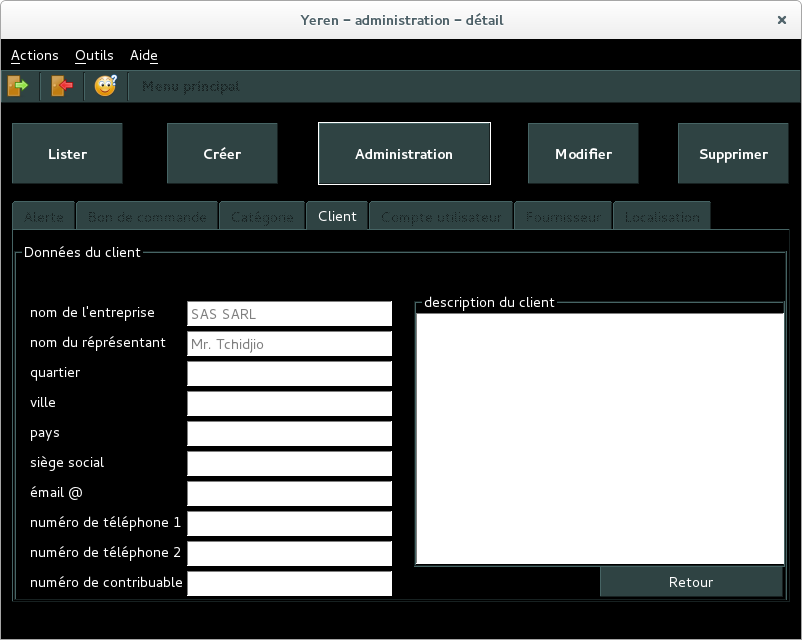
\includegraphics[scale=0.45]{images/compte-client-afficher-details.png}
	\caption{L'interface graphique pour afficher les d\'etails d'un compte client.}
	\label{fig:admin-compte-client-afficher-details}
\end{figure}

La figure~\ref{fig:admin-compte-client-afficher-details}
illustre l'interface graphique de \yeroth qui affiche les
d\'etails d'un compte client.

\procparagraph{Proc\'edure pour afficher les d\'etails d'un compte client}
\begin{enumerate}[1)]
	\item \`A partir de l'interface graphique de l'acceuil de
		l'administration (voir figure~\ref{fig:fenetre-administrateur}),
		on clique sur l'onglet intitul\'e \textbf{op\'erations}. 
		
	\item Choisir '\textbf{lister}' dans le '\emph{combo box
		op\'erations}'.
		
	\item Choisir '\textbf{un compte client}' dans le '\emph{combo box
		sujets}'. Vous \^etes automatiquement conduit \`a la fen\^etre
		illustr\'ee par la figure~\ref{fig:admin-comptes-clients-lister}.
		
	\item S\'electionner le compte client dont vous souhaitez afficher
		les d\'etails dans la liste des comptes clients affich\'ee.
		
	\item Cliquer sur le bouton \bouton{Afficher}. Les d\'etails
		du compte client sont affich\'es dans une nouvelle fen\^etre.
\end{enumerate}

%------------------------------------------------------------------------------

\newpage
\nxsubsection{Cr\'eer un compte client}\label{sec:administration-comptes-clients-lister}
\index{cr\'eer un compte client}

\begin{figure}[!htpb]
	\centering
	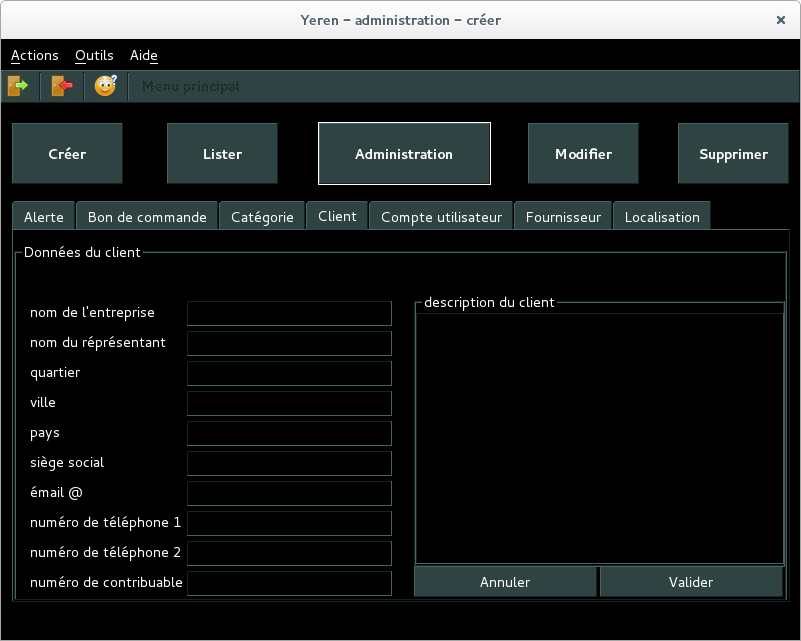
\includegraphics[scale=0.45]{images/compte-client-creer.png}
	\caption{L'interface graphique pour cr\'eer un compte client.}
	\label{fig:admin-comptes-clients-creer}
\end{figure}

La figure~\ref{fig:admin-comptes-clients-creer} illustre
l'interface graphique de \yeroth pour cr\'eer un nouveau
compte client.

\procparagraph{Proc\'edure pour cr\'eer un compte client}
\begin{enumerate}[1)]
	\item \`A partir de l'interface graphique de l'acceuil de
		l'administration (voir figure~\ref{fig:fenetre-administrateur}),
		on clique sur l'onglet intitul\'e \textbf{op\'erations}. 
		
	\item Choisir '\textbf{cr\'eer}' dans le '\emph{combo box
		op\'erations}'.
		
	\item Choisir '\textbf{un compte client}' dans
		le '\emph{combo box objets}'. Vous \^etes automatiquement
		conduit \`a la fen\^etre illustr\'ee par la
		figure~\ref{fig:admin-comptes-clients-creer}.
		
	\item Saisissez les informations requises dans les champs de texte
		suivants:
		\begin{enumerate}[1)]
			\item nom de l'entreprise \obligatoire
			\item nom du r\'epr\'esentant \obligatoire
			\item quartier
			\item ville 
			\item pays
			\item si\`ege social 
			\item \'email@ 
			\item num\'ero de t\'el\'ephone 1 
			\item num\'ero de t\'el\'ephone 2
			\item num\'ero de contribuable 
			\item description du client.			
		\end{enumerate}
		
	\item Cliquer sur le bouton \bouton{Valider} pour
		valider votre travail.		
\end{enumerate}

%------------------------------------------------------------------------------

\newpage
\nxsubsection{Lister les comptes clients}\label{sec:administration-comptes-clients-lister}
\index{lister les comptes clients}

\begin{figure}[!htpb]
	\centering
	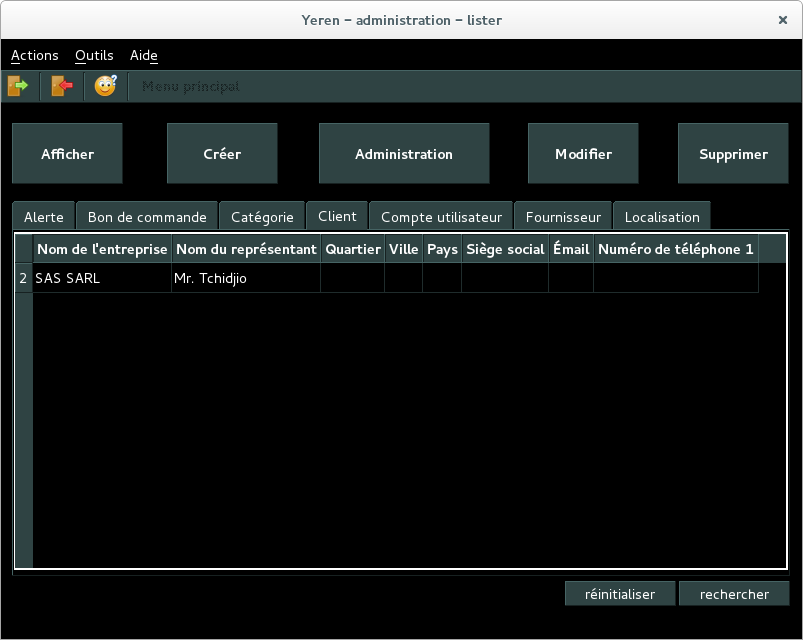
\includegraphics[scale=0.45]{images/compte-client-lister.png}
	\caption{L'interface graphique qui liste les comptes clients.}
	\label{fig:admin-comptes-clients-lister}
\end{figure}

La figure~\ref{fig:admin-comptes-clients-lister} illustre
l'interface graphique de \yeroth qui liste les comptes clients.

\procparagraph{Proc\'edure pour lister les comptes clients}
\begin{enumerate}[1)]
	\item \`A partir de l'interface graphique de l'acceuil de
		l'administration (voir figure~\ref{fig:fenetre-administrateur}),
		on clique sur l'onglet intitul\'e \textbf{op\'erations}. 
		
	\item Choisir '\textbf{lister}' dans le '\emph{combo box
		op\'erations}'.
		
	\item Choisir '\textbf{un compte client}' dans
		le '\emph{combo box objets}'. Vous \^etes automatiquement
		conduit \`a la fen\^etre qui liste les comptes clients
		(figure~\ref{fig:admin-comptes-clients-lister}).
\end{enumerate}

%------------------------------------------------------------------------------

\newpage
\nxsubsection{Modifier les d\'etails d'un compte client}
\index{modifier les d\'etails d'un compte client}

\begin{figure}[!htpb]
	\centering
	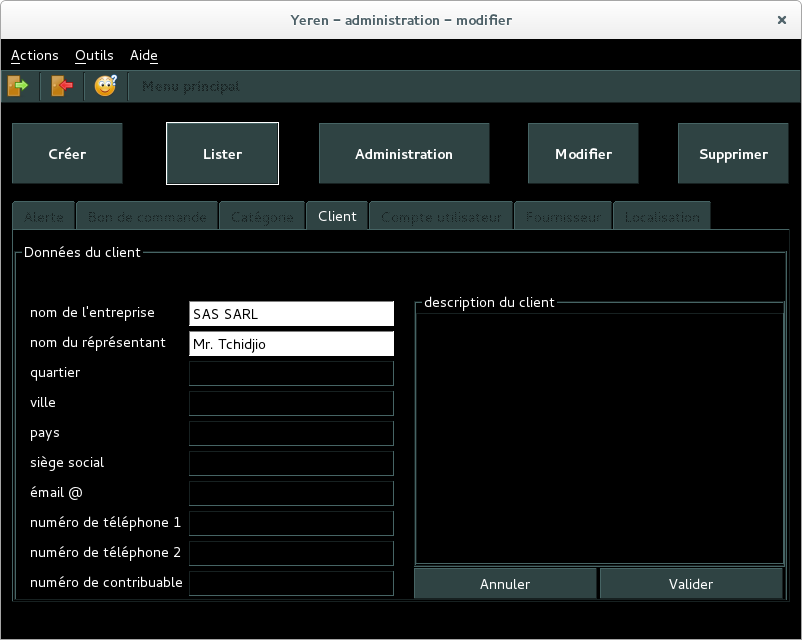
\includegraphics[scale=0.45]{images/compte-client-modifier.png}
	\caption{L'interface graphique pour modifier les d\'etails
			d'un compte client.}
	\label{fig:admin-comptes-clients-modifier}
\end{figure}

La figure~\ref{fig:admin-comptes-clients-modifier} illustre
l'interface graphique de \yeroth pour modifier les
d\'etails d'un compte client.

\procparagraph{Proc\'edure pour modifier les d\'etails d'un compte client}
\begin{enumerate}[1)]
	\item \`A partir de l'interface graphique de l'acceuil de
		l'administration (voir figure~\ref{fig:fenetre-administrateur}),
		on clique sur l'onglet intitul\'e \textbf{op\'erations}. 
		
	\item Choisir '\textbf{lister}' dans le '\emph{combo box
		op\'erations}'.
		
	\item Choisir '\textbf{un compte client}' dans le '\emph{combo box
		sujets}'. Vous \^etes automatiquement conduit \`a la fen\^etre
		illustr\'ee par la figure~\ref{fig:admin-comptes-clients-lister}.
		
	\item S\'electionner le compte client dont vous souhaitez
		modifier les d\'etails dans la liste des comptes
		clients affich\'ee.
		
	\item Cliquer sur le bouton \bouton{Modifier}. Les d\'etails
		du compte client sont affich\'es dans une nouvelle fen\^etre.
		
	\item Faites les modifications que vous souhaitez.
		
	\item Cliquer sur le bouton \bouton{valider} pour valider
		les modifications faites.
\end{enumerate}

%------------------------------------------------------------------------------

\newpage
\nxsubsection{Supprimer un compte client}
\index{supprimer un compte client}

\begin{figure}[!htpb]
	\centering
	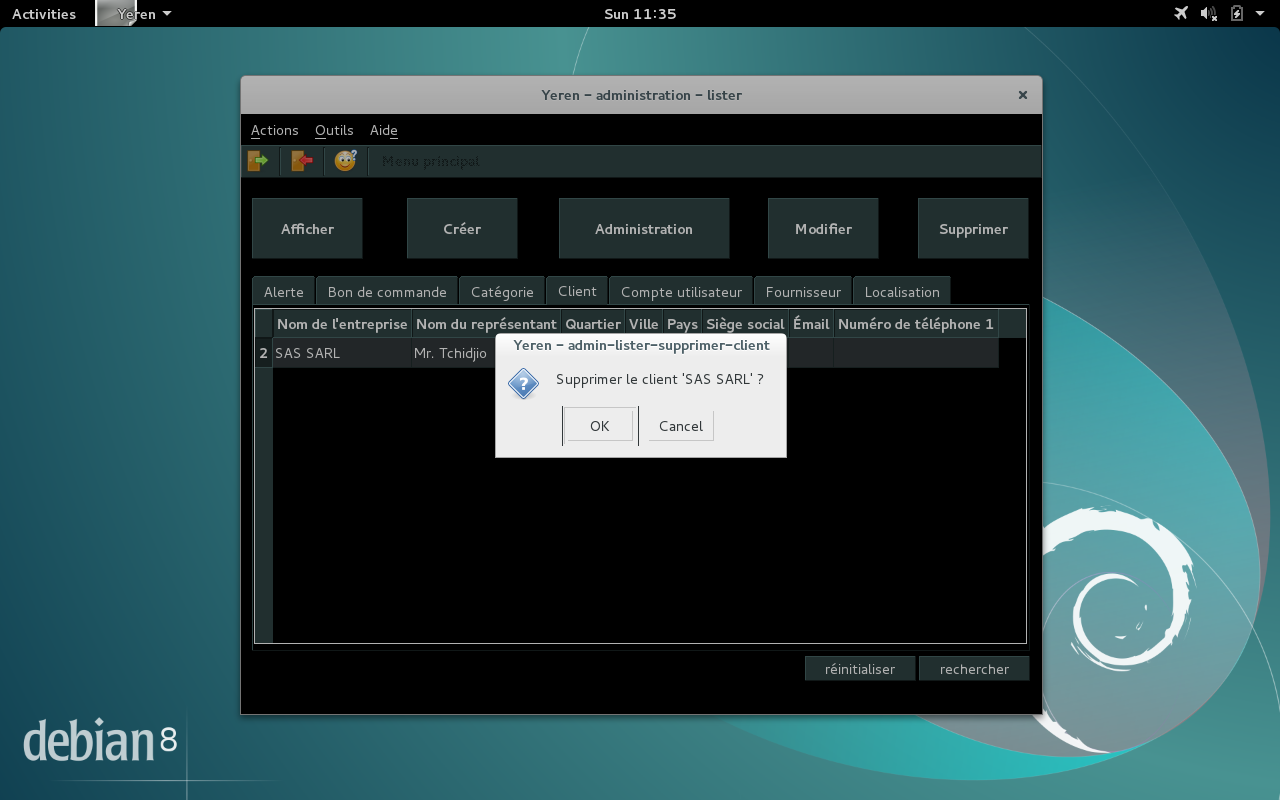
\includegraphics[scale=0.39]{images/compte-client-supprimer.png}
	\caption{L'interface graphique pour supprimer un compte client.}
	\label{fig:admin-comptes-clients-supprimer}
\end{figure}

La figure~\ref{fig:admin-comptes-clients-supprimer} illustre
l'interface graphique de \yeroth pour supprimer un compte
client.

\procparagraph{Proc\'edure pour supprimer un compte client}
\begin{enumerate}[1)]
	\item \`A partir de l'interface graphique de l'acceuil de
		l'administration (voir figure~\ref{fig:fenetre-administrateur}),
		on clique sur l'onglet intitul\'e \textbf{op\'erations}. 
		
	\item Choisir '\textbf{supprimer}' dans le '\emph{combo box
		op\'erations}'.
		
	\item Choisir '\textbf{un compte client}' dans le '\emph{combo box
		sujets}'. Vous \^etes automatiquement conduit \`a la fen\^etre
		illustr\'ee par la figure~\ref{fig:admin-comptes-clients-lister}.
		
	\item S\'electionner le compte client \`a supprimer dans la liste
		des comptes clients affich\'ee.
		
	\item Cliquer sur le bouton \bouton{Supprimer}. La question
		est ensuite pos\'ee si vous confirmer votre choix.
		Cliquer sur le \bouton{OK} pour confirmer votre choix.
\end{enumerate}
